% SIAM's class tests ifpdf for the legacy dvips-only breakurl branch.
% Tectonic/XeTeX produces PDF via xdvipdfmx, so bypass that branch while the
% unmodified class loads. Restore the actual engine test immediately after it.
% With pdfLaTeX these two compatibility files have no effect.
\RequirePackage{iftex}
\ifXeTeX
  \RequirePackage{ifpdf}
  \let\SIAMactualifpdf\ifpdf
  % Leave hyperref's engine detection intact. The class's graphics branch
  % follows immediately after hyperref and is the only test we override.
  \AddToHook{package/hyperref/after}{\let\ifpdf\iftrue}
\fi

\documentclass[review,nohypdvips,hidelinks,onefignum,onetabnum]{siamart251216}
\ifXeTeX\let\ifpdf\SIAMactualifpdf\fi

\usepackage{amsfonts,amssymb,graphicx,booktabs,array,microtype,xurl}
\usepackage{placeins,needspace,enumitem}
\setlength{\emergencystretch}{1em}
% Number every fifth line for review; adjacent display-math line numbers
% in the bundled lineno version would otherwise overlap.
\modulolinenumbers[5]
\newcommand{\creflastconjunction}{, and~}
\newsiamremark{remark}{Remark}
\newcommand{\E}{\mathbb E}
\newcommand{\Prob}{\mathbb P}
\newcommand{\R}{\mathbb R}
\newcommand{\Z}{\mathbb Z}
\newcommand{\one}{\mathbf 1}
\newcommand{\W}{W_1}
\newcommand{\eps}{\varepsilon}
\newcommand{\gb}{\overline g}
\newcommand{\TV}{\operatorname{TV}}
\newcommand{\cL}{\mathcal L}
\newcommand{\sh}{\mathsf S}
\newcommand{\dd}{\,\mathrm d}
\newcommand{\norm}[1]{\left\lVert#1\right\rVert}
\DeclareMathOperator{\diag}{diag}
\headers{Critical Overflow in Two-Choice Allocation}{Silas Lu}
\title{Critical Overflow in Weakly Coupled Two-Choice Allocation}
\author{Silas Lu\thanks{School of Information Management, Nanjing University,
Nanjing, China. ORCID: \href{https://orcid.org/0009-0005-1387-2849}{0009-0005-1387-2849}.}}

\externaldocument[][nocite]{../output/pdf/supplement_sicomp}[supplement_sicomp.pdf]
\hypersetup{pdftitle={Critical Overflow in Weakly Coupled Two-Choice Allocation},pdfauthor={Silas Lu}}
\begin{document}
\maketitle
\begin{abstract}
We determine which candidate information a reduced model must retain to predict
critical overflow in a fixed two-choice allocation rule.
Two communities of $q$ buckets have uniform bipartite internal sampling and
cross sampling of probability $\eps$. Each cross direction uses a predetermined
doubly stochastic kernel; ties favor the left endpoint.
For empty starts, $\eps q\to\lambda<\infty$, and integer capacity $c$ with
$2c/q\to\kappa>0$, we prove a common joint limit for imbalance and the
overflow curve on the $q^2$ arrival scale.
A coupling compares the actual fixed-kernel and product processes.
An exact midpoint evolution proves attraction to a unique two-side lattice profile.
The imbalance converges to a scalar diffusion whose drift averages the fast
common phase. Overflow retains the observation phase and the internal profile.
Community excess alone therefore misses a positive order-$q$ contribution to
expected overflow. At nominal capacity, expected overflow is order $q$,
while its fraction tends to zero.
Joint first Wasserstein convergence justifies both distributional and mean conclusions.
Certified profile evaluation and preserved samples assess the separate prediction
steps at specified finite-size tolerances. No effective uniform error bound
for the joint critical limit is asserted.
\end{abstract}
\begin{keywords}
randomized allocation, two choices, graphical load balancing, overflow,
universality, diffusion approximation
\end{keywords}
\begin{MSCcodes}
68W20, 60F17, 60C05
\end{MSCcodes}
\section{Introduction}\label{sec:intro}
Two-choice allocation assigns each item to the less loaded of two
candidates~\cite{azar}. We study the total number of items assigned beyond
bucket capacity. At total nominal capacity, overflow equals half the total
absolute deviation from capacity. Its prediction requires information beyond
the largest load.

We ask which information a reduced model must retain for two weakly coupled
communities. Each community has $q$ buckets with uniform internal bipartite
candidates. A fraction $\eps$ of candidates connect the communities through
any predetermined doubly stochastic kernel. Both fixed matchings and product
sampling have the required uniform endpoint marginals.
Ties favor the left endpoint, as in the internal two-group
Always-Go-Left rule of V\"ocking~\cite{vocking}.

With empty starts and integer capacity $c\asymp q$, critical fill occurs at
$n_*=2qc\asymp q^2$ arrivals. Without cross sampling, community choices
produce order-$q$ imbalance fluctuations. Cross arrivals can contribute order
$\eps q$ to the cumulative normalized drift. These scales motivate weak
coupling $\eps q\to\lambda<\infty$.

Every admissible fixed cross kernel has the same first-order critical law.
Internal load variation remains in that law, even at known community imbalance.
Expected overflow is order $q$, while its fraction of arrivals tends to zero.
Changing the fixed cross kernel preserves its leading coefficient.

Figure~\ref{fig:profileablation} shows the missing internal contribution.
Section~\ref{sec:experiments} separates this readout comparison from the
unconditional diffusion test.

\begin{figure}[t]
\centering
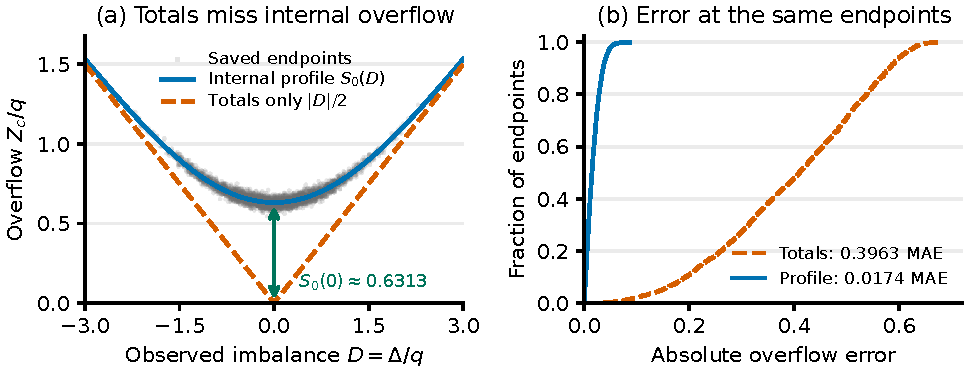
\includegraphics[width=\textwidth]{figures/readout_teaser.pdf}
\caption{Community totals miss internal overflow at critical fill.
Left: 4096 saved endpoints at $q=512$, $\kappa=1$, $\lambda=1$, with matching
crosses. The profile curve retains internal variation; $|D|/2$ uses only
community excess. Their gap at $D=0$ is approximately $0.6313$.
Right: absolute-error distributions for the same endpoints, with mean absolute
errors in the legend. Both readouts use the observed imbalance.
This is a descriptive mechanism comparison; the separate terminal test checks
the diffusion. The frozen profile lookup error is at most $0.000026$.}
\label{fig:profileablation}
\end{figure}

\subsection{Contributions}
Theorems~\ref{thm:universal}--\ref{thm:limit} establish three linked results.
\begin{enumerate}[label=(\roman*),leftmargin=*]
\item \textbf{Comparison of the actual allocation processes.}
For any predetermined doubly stochastic cross kernels, we couple the genuine
fixed-kernel process to the genuine product process. On each fixed $Tq^2$
horizon, their four sorted side vectors have expected uniform $\ell_1$
distance $O_{T,\Lambda}(q^{5/6}\log^2q)$ when $\eps q\le\Lambda$.
The bound controls imbalance and overflow at all common capacities.
Random-label forgetting first controls the whole cross load-pair table.
A coupling of sorted ranks then preserves the laws of both actual processes.
\item \textbf{An attracting internal lattice profile.}
We construct a unique mean-locked periodic family for the two-side tail flow.
It has full support, exponential moments, and uniform attraction on fixed
centered exponential-moment sublevels. An exact positive midpoint evolution
of signed tail differences gives strict contraction on equal-mean slices.
Its half-phase left/right identity records the asymmetric tie rule.
\item \textbf{A joint critical law for imbalance and overflow.}
For $\eps q\to\lambda$, normalized imbalance converges to a scalar diffusion.
Its restoring drift averages the fast common lattice phase.
The overflow curve retains the observation phase of the same internal profile.
Joint first Wasserstein convergence controls expected overflow as well as laws.
Corollaries~\ref{cor:internalexcess} and~\ref{cor:capacity} give the omitted
internal contribution and its capacity consequences.
\end{enumerate}
The capacity corollaries interpret the joint law for the fixed rule.

\subsection{Relation to previous work}
\textit{Existing rules and distribution equations.}
V\"ocking~\cite{vocking} introduced Always-Go-Left.
Berenbrink, Czumaj, Steger, and V\"ocking~\cite{bcsv} give sharp heavy-load
deviation bounds for greedy and asymmetric allocation.
Mitzenmacher~\cite{mitzode} uses differential equations to describe full load
distributions. We use this established distribution-level viewpoint.
The additional requirements here are long-time attraction of a two-type
integer-lattice profile and its coupling to a slow community imbalance.

\textit{Correlated choices and process comparison.}
Mitzenmacher~\cite{doublehash,doublecoupling} shows asymptotic equivalence
between double hashing and fully random balanced allocation, using fluid
limits and a coupling through a biased intermediate process.
The stated distribution results concern a constant number of choices and
$TN$ arrivals into $N$ bins for fixed $T$.
Our comparison treats arbitrary fixed doubly stochastic cross kernels,
allows only order-$q^{-1}$ cross probability, and covers $Tq^2$ arrivals.
It bounds the distance between the genuine fixed-kernel and product processes.
These differences are needed before passing to the critical overflow law.

\textit{Graphs and queues.}
Peres, Talwar, and Wieder~\cite{ptw} study graphical allocation and limited
choice. Bansal and Feldheim~\cite{bf} give a strategy based on graph
decompositions. Our rule compares only the two endpoint loads.
Queueing universality and diffusion limits~\cite{universality,bmw,atar}
include service and use different scales. Here each item has two candidates
and loads only increase.

\textit{Traveling profiles.}
Stolyar~\cite{stolyarwave,stolyarstationary} develops traveling-wave and
stationary-limit methods. Contraction and compactness are precedents.
The existence result in~\cite[Theorem 3]{stolyarwave} permits general jumps.
Its uniqueness and attraction result~\cite[Theorem 4]{stolyarwave} requires
a positive jump density bounded away from zero on compact subsets of
$\R_+$. The arithmetic-jump caveat following that theorem prevents its direct
use for the present lattice dynamics. We prove the two-side periodic-family
result directly, then obtain finite-system tracking without a stationary-limit
interchange. The later phase averaging acts on the slow drift, while the
critical overflow retains its endpoint phase.

Sections~\ref{sec:model}--\ref{sec:limit} state and prove the results.
Section~\ref{sec:experiments} evaluates their prediction steps.
The supplement gives numerical certificates, statistical protocols, and provenance.

\section{Model and main results}\label{sec:model}
There are communities $C_0=L_0\cup R_0$ and $C_1=L_1\cup R_1$, each side of size $m$, and $q=2m$. At each arrival choose an internal edge in $C_s$ with probability $(1-\eps)/2$, for each $s$, or direction $L_0$--$R_1$ or $L_1$--$R_0$ with probability $\eps/2$ each. Internal edges are uniform on $K_{m,m}$. In cross direction $d$, a fixed nonnegative matrix $B^{(d)}$ has all row and column sums one; conditional edge probability is $B^{(d)}_{ij}/m$. Product sampling has $B=J/m$ and a matching is a permutation matrix. Matrices may depend deterministically on $q$. A randomly selected matrix is admissible if chosen independently before the arrivals, by conditioning on it. Matrices selected from current loads are excluded.

Loads $A_v(n)$ are nonnegative integers, initially zero. Increment the endpoint of smaller load, breaking every tie to the left side. Let
\[
 M_s(n)=\sum_{v\in C_s}A_v(n),\quad \Delta_n=M_0(n)-M_1(n),
 \quad Z_c(n)=\sum_v(A_v(n)-c)_+.
\]
For integer $c$, $Z_c$ is also the number of overflows when each bucket stores its first $c$ assigned items. Indeed the capped loads remain $\min(A_v,c)$ under the same candidate stream: below capacity both comparisons agree, and once both candidates are full the uncapped winner is irrelevant to the overflow count. This identifies the overflow count with the positive-part load functional.

For a pair of integer laws $z=(p_L,p_R)$ with finite first moments, write
\[
 x_k=p_L([k,\infty)),\quad y_k=p_R([k,\infty)),\quad
 a_k=x_k-x_{k+1},\quad b_k=y_k-y_{k+1},
\]
and $\mu(z)=(\E L+\E R)/2$. The metric $d_1$ is the sum of the two marginal Wasserstein distances, equivalently the sum of absolute tail differences. Integer shift $\sh_j$ adds $j$ to both laws.


There are three time scales. After $k$ internal arrivals in one community,
its mean clock is $u=k/q$. The common mean at global arrival $n$ is
$h_n=n/(2q)$. The slow diffusion clock is $t=n/q^2$.
At critical fill $n_*=2qc=4mc$, these give $h_{n_*}=c$ and
$n_*/q^2=c/m\to\kappa$. An offset of $2hq$ arrivals changes the common mean
by $h$ while changing slow time by only $2h/q$.
Figure~\ref{fig:model} shows the candidate structure and the two retained states.

\begin{figure}[t]
\centering
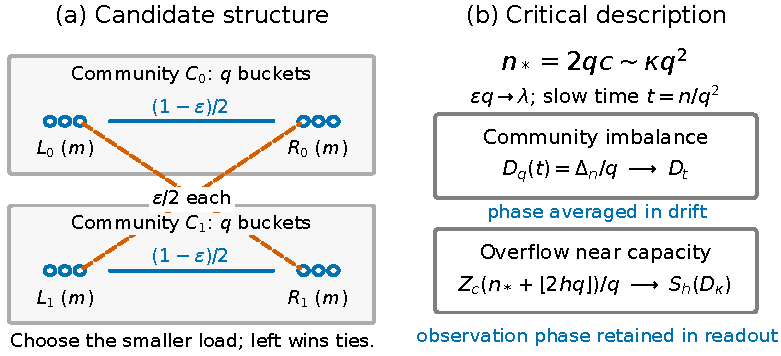
\includegraphics[width=\textwidth]{figures/model_scales.pdf}
\caption{The fixed allocation rule and its critical scales. Each of the four
sides contains $m=q/2$ buckets. Internal directions have probability
$(1-\eps)/2$ each; cross directions have probability $\eps/2$ each.
The offered cross endpoints have uniform marginals under any fixed doubly
stochastic kernel. The algorithm increments the smaller endpoint load and
chooses the left endpoint at a tie. The limiting diffusion retains community
imbalance; the overflow readout also retains the internal profile.}
\label{fig:model}
\end{figure}


For integer capacities $c_q$, set
\[
 n_*=2qc_q,\qquad n_q(h)=n_*+\lfloor2qh\rfloor.
\]
When $c_q/m\to\kappa>0$, each bounded $h$ window has nonnegative indices for large $q$.
The imbalance path $D_q$ linearly interpolates $\Delta_n/q$ at times $n/q^2$.
The overflow curve $F_q$ linearly interpolates $Z_{c_q}(k)/q$ at coordinates
$h=(k-n_*)/(2q)$. Its distance from $Z_{c_q}(n_q(h))/q$ is at most $1/q$.

All path and curve Wasserstein distances below have order one. They use the uniform norm on the corresponding continuous-function space. Joint convergence uses the sum of the path and curve uniform norms. Thus, for a metric $d$, the transport distance is $\inf\E d(U,V)$ over couplings with the stated laws.

\Needspace{10\baselineskip}
\begin{theorem}[Fixed-kernel universality]\label{thm:universal}
For empty starts and fixed $T,\Lambda<\infty$, assume $q\ge4$, $\eps\le1/4$ and $\eps q\le\Lambda$. A genuine fixed-kernel process and a genuine product process admit a coupling such that, for $\mathcal D_n$ the sum of absolute differences of their four separately sorted side vectors,
\[
 \E\max_{n\le Tq^2}\frac{\mathcal D_n}{q}
 =O_{T,\Lambda}(q^{-1/6}\log^2q)\longrightarrow0.
\]
The same bound controls $|\Delta^F-\Delta^P|/q$ and $|Z_c^F-Z_c^P|/q$, simultaneously for all common capacities $c\ge0$.
\end{theorem}

\Needspace{12\baselineskip}
\begin{theorem}[Internal periodic profile]\label{thm:profile}
The mean-clock tail flow
\begin{equation}\label{eq:flow}
 \dot x_k=2a_{k-1}y_{k-1},\qquad
 \dot y_k=2b_{k-1}x_k
\end{equation}
has a unique finite-first-moment periodic family $\rho^u=(L_u,R_u)$ with mean $u$, satisfying
\[
 \rho^{u+1}=\sh_1\rho^u,\qquad \Phi_t\rho^u=\rho^{u+t}.
\]
It has exponential moments, full support at every integer, and
$d_1(\rho^u,\rho^v)=2|u-v|$. Attraction is uniform over centered exponential-moment sublevels and all initial phases. No effective attraction rate is asserted.
\end{theorem}

Define independent-draw comparisons and the overflow readout by
\begin{align}
 H(u,v)&=\Prob(L_u\le R_v),\nonumber\\
 g(h,d)&=H(h+d/2,h-d/2)-H(h-d/2,h+d/2),\label{eq:g}\\
 \gb(d)&=\int_0^1g(h,d)\dd h,\nonumber\\
 \sigma(u)&=\tfrac12\{\E(L_u)_++\E(R_u)_+\},\quad
 S_h(d)=\sigma(h+d/2)+\sigma(h-d/2).\label{eq:spill}
\end{align}

\Needspace{19\baselineskip}
\begin{theorem}[Common critical limit]\label{thm:limit}
If $\eps q\to\lambda\in[0,\infty)$, then for every fixed $T$, $D_q\to D$ in first Wasserstein distance for the uniform path norm on $[0,T]$, where
\begin{equation}\label{eq:sde}
 \dd D_t=\dd B_t+\lambda\gb(D_t)\dd t,\qquad D_0=0.
\end{equation}
The function $\gb$ is odd, smooth, strictly decreasing, globally $2$-Lipschitz and negative on $(0,\infty)$, with $\gb'(0)<0$ and $\gb(d)\to-\operatorname{sign}(d)$ at infinity. Let the integer capacities satisfy $c_q/m\to\kappa\in(0,\infty)$. For each $H_0<\infty$ and $T_*>\kappa$,
\[
 \bigl(D_q|_{[0,T_*]},F_q|_{[-H_0,H_0]}\bigr)
 \longrightarrow
 \bigl(D|_{[0,T_*]},(S_h(D_\kappa))_{|h|\le H_0}\bigr)
\]
in first Wasserstein distance for the sum of the two uniform norms. Restriction gives joint convergence with any shorter path horizon. This holds for every fixed kernel above. The function $S_h$ is even and convex in $d$, $1$-Lipschitz in $d$, and $2$-Lipschitz in $h$, with $S_0(0)>0$.
\end{theorem}

The drift averages the common phase along many complete cycles. The overflow
readout at the integer critical count has phase zero and is not phase averaged.
The function $S_h$ is not periodic in $h$: the observation offset changes the
fill level as well as the lattice phase. Theorem~\ref{thm:universal} gives an
explicit but conservative kernel-comparison bound. The joint critical limit
has no effective uniform finite-size error bound.

Figure~\ref{fig:mechanism} displays the profile and averaged response.

\begin{figure}[t]
\centering
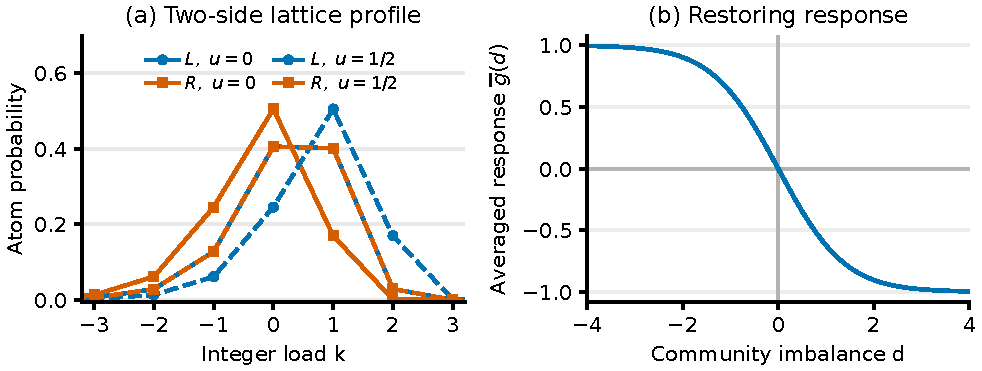
\includegraphics[width=\textwidth]{figures/profile_mechanism.pdf}
\caption{Internal structure and restoring response, replotted from saved
profile nodes and the frozen response table. Left: left and right atom
probabilities at mean phases $u=0$ (solid) and $u=1/2$ (dashed).
Only the displayed load levels are shown. The half-phase operation swaps
the sides and shifts the new left law by one. Right: the phase-averaged
response $\gb(d)$; positive imbalance has negative response.
Connecting segments are for display. No new trajectory or numerical solution
enters this figure.}
\label{fig:mechanism}
\end{figure}

\begin{corollary}[A leading internal overflow contribution]\label{cor:internalexcess}
Under Theorem~\ref{thm:limit}, fix $\kappa>0$ and $\lambda<\infty$. Let $X_u$ have the equal mixture of the two laws in $\rho^u$, and set
\[
 r(u)=\E(X_u)_+-u_+=\tfrac12(\E|X_u|-|u|).
\]
Then $r(u)>0$ for every finite $u$, and
\[
 S_0(d)=\frac{|d|}{2}+r(d/2)+r(-d/2).
\]
For every admissible fixed cross kernel,
\[
 \lim_{q\to\infty}\E\left[\frac{Z_{c_q}(n_*)-|\Delta_{n_*}|/2}{q}\right]
 =\E\{r(D_\kappa/2)+r(-D_\kappa/2)\}>0.
\]
The positive limit may depend on $\kappa$ and $\lambda$.
\end{corollary}
\begin{proof}
The mixture has mean $u$. Full support from Theorem~\ref{thm:profile} gives positive mass on both sides of zero. Hence $\E|X_u|>|\E X_u|=|u|$. Substitution into \eqref{eq:spill} gives the displayed decomposition.

At $n_*=2qc_q$, the community excess totals are $\Delta_{n_*}/2$ and $-\Delta_{n_*}/2$. Taking positive parts within each community yields the exact finite-size inequality $Z_{c_q}(n_*)\ge|\Delta_{n_*}|/2$. Put $\kappa_q=n_*/q^2\to\kappa$. The endpoint-time estimate \eqref{eq:endpointtime} shows $\E|D_q(\kappa_q)-D_q(\kappa)|\to0$. The joint first Wasserstein convergence in Theorem~\ref{thm:limit} therefore passes expectations for the Lipschitz, linear-growth difference readout. This gives the stated limit. Its integrand is strictly positive at every finite value of $D_\kappa$, and its expectation is finite.
\end{proof}

This corollary identifies the information omitted by an imbalance-only approximation. It follows from the profile and critical-limit theorems. It does not assert a uniform positive gap over all parameters. The imbalance-only readout is a mechanistic simplification, rather than a claimed strongest published competitor.

\begin{corollary}[Capacity consequences]\label{cor:capacity}
Under Theorem~\ref{thm:limit}, let $s_*=S_0(0)>0$ and
$C_{\kappa,\lambda}=\E S_0(D_\kappa)$. For each fixed $a\in(0,s_*)$,
\[
 \Prob\{Z_{c_q}(n_*)\ge aq\}\longrightarrow1,
 \qquad \Prob\{Z_{c_q}(n_*)=0\}\longrightarrow0.
\]
Moreover,
\[
 \E Z_{c_q}(n_*)=qC_{\kappa,\lambda}+o(q),\qquad
 \frac{\E Z_{c_q}(n_*)}{n_*}
 =\frac{C_{\kappa,\lambda}}{\kappa q}+o(q^{-1}).
\]
These conclusions and their leading coefficient hold for every admissible
fixed cross kernel.
\end{corollary}
\begin{proof}
Evenness and convexity give $S_0(d)\ge S_0(0)>a$ for every $d$.
Weak convergence of $Z_{c_q}(n_*)/q$ and the open-set inequality therefore give
the probability limits. First Wasserstein convergence passes its expectation
to $C_{\kappa,\lambda}<\infty$. Finally, $n_*/q^2\to\kappa>0$ gives the
fractional asymptotic. The common limit is independent of the fixed cross kernel.
\end{proof}

Kernel choice within the stated class does not remove the leading overflow
cost. This consequence of the joint law does not compare other allocation strategies.

\section{From a fixed cross kernel to product sampling}\label{sec:universality}
This section proves Theorem~\ref{thm:universal} by coupling the actual processes.
Internal sampling first forgets a random label transposition under a dispersion
bound. This controls the whole cross load-pair table.
A sorted-rank coupling then uses greedy nonexpansion.
Fix $\theta=1/200$, $K_0=16/3$, and $I=(1-\eps)/2$.
The constants are conservative.

\begin{figure}[t]
\centering
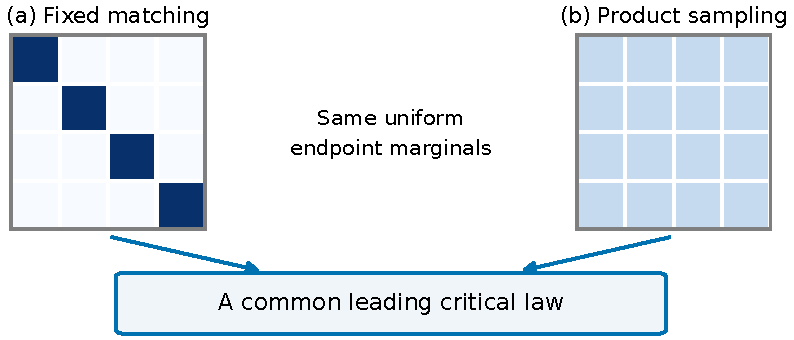
\includegraphics[width=\textwidth]{figures/kernel_universality.pdf}
\caption{Different fixed cross correlations share the critical law under the
model and scaling of Theorems~\ref{thm:universal}--\ref{thm:limit}.
The grids show conditional candidate-pair probabilities in one cross direction,
with four illustrative labels on each side. Matching probabilities are $1/4$
on the diagonal and zero elsewhere; product probabilities are all $1/16$.
Both have uniform marginals. Internal sampling and rare cross arrivals are
essential to the theorem; uniform marginals alone do not imply independent loads.}
\label{fig:kernels}
\end{figure}

\begin{lemma}[Dispersion]\label{lem:moment}
With $\xi_v=A_v-M_{s(v)}/q$ and $\Gamma=\sum_v\cosh(\theta\xi_v)$, every fixed uniform-marginal kernel satisfies
\begin{equation}\label{eq:moment}
 \sup_{n\ge0}\E\Gamma_n\le K_0q.
\end{equation}
\end{lemma}
\begin{proof}
The rank-based potential argument is given in Supplement
section~\ref*{app:dispersion}. It uses only the cross marginals.
\end{proof}

\begin{lemma}[Random transposition]\label{lem:swap}
Let $\mu_n$ be the law of the actual fixed-kernel configuration. Independently choose two uniform labels $i,j$ in one side, and let $\tau$ swap them. For $\ell\ge4$, integer $L=q\ell$, and $n\ge L$,
\begin{align}
 \E_{i,j}\TV(\mu_n,\tau\mu_n)&\le\eta,\label{eq:eta}\\
 \eta&=\min\left\{1,\frac{32K_0}{\theta\sqrt\ell}
 +16K_0e^{-\theta\ell/16}+e^{-L/48}+4\eps\ell\right\}.\nonumber
\end{align}
\end{lemma}
\begin{proof}
Compare the original and transposed configurations through the conjugate
kernel. The two discrepancies behave as tags until they meet.
Suppress cross events touching a tag; internal updates then make the tag gap
no harder to absorb than a fair walk. Dispersion controls the initial gap
and deviations at the window endpoints. On the remaining event, nonmeeting
requires at least $\lceil\ell/4\rceil$ embedded jumps.
A fixed-jump reflection bound gives the first term of $\eta$.
The conjugate-kernel comparison adds a second cross-touch allowance.
Supplement section~\ref*{app:swapdetails} gives the full coupling and constants;
it does not condition a martingale estimate on a future jump count.
\end{proof}

For one cross direction write $Q_n$ for its actual conditional joint load-pair law and $p_n,r_n$ for the empirical side marginals. If $0\le f\le1$, define
\[
 C_B(f)=\frac1m\sum_{ij}B_{ij}f(U_i,V_j)
       -\frac1{m^2}\sum_{ij}f(U_i,V_j).
\]
The test may use parameters unchanged by the side swap, including community
means. Let $I_0$ be uniform, draw $J_0\mid I_0$ from the corresponding row
of $B$, and draw $J'_0$ independently and uniformly. We claim
\begin{equation}\label{eq:correlation}
 \E C_B(f)^2\le2\eta+2/m,
 \qquad \E|C_B(f)|\le\sqrt{2\eta+2/m}.
\end{equation}
Write $C=C_B(f)$ and take these auxiliary indices independently of the
configuration. Pointwise,
\[
 C^2=\E_{\rm aux}\bigl[C\{f(U_{I_0},V_{J_0})-f(U_{I_0},V_{J'_0})\}\bigr].
\]
For fixed indices let $\tau$ exchange $J_0,J'_0$. The product-marginal term of $C$ is unchanged, and $|C(\tau A)-C(A)|\le2/m$. Apply total variation to $G(A)=C(A)f(U_{I_0},V_{J_0})$, for which $|G|\le1$. Thus the expected difference is at most $2\TV(\mu_n,\tau\mu_n)+2/m$. After averaging, $(J_0,J'_0)$ are independent uniform side labels: column sums make $J_0$ uniform, even though it depends on $I_0$. Lemma~\ref{lem:swap} gives \eqref{eq:correlation}. The bounded-test TV cost is $2\eta$. This controls the second moment, rather than only a signed average.

Center each load coordinate at its community's integer mean part. For each fixed offset cell in $[-R,R]^2$, its indicator satisfies \eqref{eq:correlation}. Summing over this deterministic square and using \eqref{eq:moment} outside it yields
\begin{equation}\label{eq:rho}
 \E\norm{Q_n-p_n\otimes r_n}_1\le\rho,
 \quad \rho=\min\{2,(2R+1)^2\sqrt{2\eta+2/m}
                      +16K_0e^{-\theta(R-1)}\}.
\end{equation}
Indeed $Q$ and the product have the same marginals; twice their marginal tail masses bounds the mass outside the square. Replacing the mean by its integer part costs at most one in the exponential bound. No supremum over arbitrary data-dependent tests is taken.

It remains to compare two actual process laws. Sort each side separately. Integer greedy updates using the same offered ranks are nonexpansive in sorted $\ell_1$ distance: if different winners are chosen, the two relevant coordinate differences have the ordering needed for their $+1,-1$ changes not to increase the absolute sum; sorting again minimizes the matching cost. Internally use common independent uniform ranks. At a cross, sample the actual fixed edge in the fixed process, then maximally couple its load pair from $Q_F$ to a virtual pair from $p_F\otimes r_F$. Given the virtual loads, choose ranks independently and uniformly inside the equal-load blocks. Conditional on the entire joint past before drawing the current edge, these ranks are independent uniforms, since a block of size $k$ has mass $k/m$ followed by probability $1/k$ per rank. Use the same ranks in the product process, which therefore has its genuine transition law. Independence need not persist after additionally conditioning on the current realized fixed edge.

On successful load-pair coupling the actual and virtual sorted fixed-process updates agree, including ties. On failure their distance is at most two. Hence
\[
 \mathcal D_{n+1}\le\mathcal D_n+
 2\one_{\{\text{cross and load-pair coupling fails}\}}.
\]
Before $L$ use failure probability one; afterwards its expected conditional value is at most $\rho/2$. Summing the nonnegative counts gives the explicit bound
\begin{equation}\label{eq:finitecoupling}
 \E\max_{n\le N}\mathcal D_n
 \le2\eps\min(N,L)+\eps\rho(N-L)_+.
\end{equation}
Take $\ell=\max(4,\lceil q^{2/3}\rceil)$ and $R=\lceil(2/\theta)\log q\rceil+1$. Then \eqref{eq:finitecoupling} divided by $q$, for $N\le Tq^2$, is $O(q^{-1/6}\log^2q)$. Both the community difference and every positive-part sum are $1$-Lipschitz in sorted load distance. This proves Theorem~\ref{thm:universal}. The bound is asymptotic and extremely conservative; it is not a numerical error bar at the experimental sizes.

\section{The mean-locked internal orbit}\label{sec:profile}
The main step is an exact midpoint equation for the difference of two tail
flows. It gives strict contraction on equal-mean slices without uniform
irreducibility on the whole lattice. Compactness then yields the periodic
family and uniform attraction on each fixed moment sublevel.
In this section all times use the mean clock. Signed lattice coordinates express translated laws; actual allocations remain nonnegative. Equation~\eqref{eq:flow} has a unique probability flow on finite-first-moment laws. It can be constructed by two coupled bounded-rate birth laws with left rate $2y_k$ and right rate $2x_{k+1}$. Picard iteration, or finite truncation followed by tightness, gives existence and uniqueness. The tail field is globally Lipschitz, probability constraints are invariant, and rates at most two prevent explosion. The sum of the mean derivatives is two, so $\mu(\Phi_tz)=\mu(z)+t$.

\subsection{Moment compactness and exact nonexpansion}
Let
\[
 V_\theta(z)=\E\cosh(\theta(L-\mu))+\E\cosh(\theta(R-\mu)).
\]
The selected-load distribution is $w_k=a_ky_k+b_kx_{k+1}$, of total mass one, bounded by twice the pooled law $\nu=(p_L+p_R)/2$. Its suffix is $x_ky_k\le[(x_k+y_k)/2]^2$. The same rank/Gini argument as in Lemma~\ref{lem:moment}, now with pure-internal rank deficit one, and differentiation of the moving mean give
\begin{equation}\label{eq:fluidmoment}
 \frac\dd{\dd t}V_\theta(\Phi_tz)
 \le-\{\theta/2-2(e^\theta-1-\theta)\}V_\theta+\theta
 \le-\theta V_\theta/4+\theta.
\end{equation}
Truncation justifies this calculation for finite exponential moments. Thus every centered sublevel $V_\theta\le M$, $M\ge4$, is invariant. No attraction theorem is used to obtain this bound.

For two solutions put $d_k=x_k-\widetilde x_k$, $e_k=y_k-\widetilde y_k$, and let bars denote midpoint tails or atoms. Their difference satisfies exactly the forward equation on states $X_k,Y_k$ with transitions
\begin{align*}
 X_k&\longrightarrow X_{k+1} &&\text{at rate }2\bar y_k,&
 X_k&\longrightarrow Y_k &&\text{at rate }2\bar b_{k-1},\\
 Y_k&\longrightarrow Y_{k+1} &&\text{at rate }2\bar x_{k+1},&
 Y_k&\longrightarrow X_{k+1} &&\text{at rate }2\bar a_k.
\end{align*}
Exit rates are $2\bar y_{k-1}$ and $2\bar x_k$, at most two. The midpoint identity is exact for the bilinear field, with no discarded remainder. Its evolution is positive and mass preserving, so
\begin{equation}\label{eq:nonexp}
 d_1(\Phi_tz,\Phi_t\widetilde z)\le d_1(z,\widetilde z).
\end{equation}
It also shows that the field is $4$-Lipschitz in tail $\ell_1$.

\subsection{Strictness on an equal-mean slice}
Positivity needed for strictness must be checked, since the generator need not be irreducible initially. Choose one positive atom on each side. Atoms retain at least $e^{-2t}$ of their initial mass. If a left atom is below a right atom, the left can advance to one above it through positive birth flux, after which the right can advance. If the left begins above the right, advance the right first. Variation of constants and induction show that every sufficiently high atom on each side is positive for every $t>0$. Consequently every finite tail is positive at positive times.

In the midpoint chain, all same-channel forward edges at finite levels therefore have positive rates, and both crossing types are positive at sufficiently high levels. Any two finite starting states can reach a common high $X_K$ in a positive time interval with positive probability: choose a finite path in a compact subinterval of $(0,t)$ and use positive continuous rates there, together with the bounded waiting rates. This is a pointwise argument, with no uniform minorization over the whole lattice.

If two distinct initial laws have the same mean, the summable signed tail difference has zero total mass and both signs. Choose one coordinate of each sign. Positive portions of their transported masses overlap at the common high state, causing strict cancellation. Hence for every $t>0$,
\begin{equation}\label{eq:strict}
 d_1(\Phi_tz,\Phi_t\widetilde z)<d_1(z,\widetilde z)
 \quad\text{if }\mu(z)=\mu(\widetilde z),\ z\ne\widetilde z.
\end{equation}

\subsection{Existence, uniqueness and uniform attraction}
On a fixed mean slice define $T=\sh_{-1}\Phi_1$. The set
$\{\mu=\alpha,V_\theta\le M\}$ is compact in $d_1$: exponential tails imply tightness and uniform integrability of first moments; the moment sublevel is closed by lower semicontinuity. It is nonempty for sufficiently large $M$, uniformly for $\alpha\in[0,1]$, using identical mixtures on $\{0,1\}$. The map $T$ is continuous, preserves the set, and strictly decreases distances between distinct points.

Here is the compact argument explicitly. Along an orbit, consecutive distances decrease to $r$. A convergent subsequence with limit $z$ gives both $d_1(z,Tz)=r$ and $d_1(Tz,T^2z)=r$. Strictness forces $r=0$, hence a fixed point. Two fixed points contradict strictness. The distance from any orbit to that point decreases; a second subsequence argument forces convergence to zero. On the compact set the continuous distance functions decrease pointwise to zero, so a finite-subcover argument makes the convergence uniform. Fixed points in nested sublevels agree.

Let $z_*$ be the mean-zero fixed point and define
\[
 \rho^u=\sh_{\lfloor u\rfloor}\Phi_{\{u\}}z_*.
\]
The flow and period identities follow, with $V_\theta(\rho^u)\le4$ by \eqref{eq:fluidmoment}. Any other finite-first-moment periodic family would keep its equal-mean distance to this one unchanged over a period, contradicting \eqref{eq:strict}. Thus uniqueness extends beyond the exponential class used for construction.

For each fixed $M\ge4$, the set $K_M=\{z:\mu(z)\in[0,1],\ V_\theta(z)\le M\}$ is compact in $d_1$. The moment bound $M$ remains fixed in this argument. The target $\rho^{\mu(z)}$ is continuous because the phase endpoints match. Applying the same decreasing-function compactness argument, and using nonexpansion between integer times, gives
\begin{equation}\label{eq:omega}
 \omega_M(t):=\sup_{\substack{\mu(z)\in[0,1]\\V_\theta(z)\le M}}
 d_1(\Phi_tz,\rho^{\mu(z)+t})\longrightarrow0.
\end{equation}
Integer translation covers arbitrary means. Along the birth flow each side increases stochastically. Summing the two mean increments therefore gives
\begin{equation}\label{eq:geometry}
 d_1(\rho^u,\rho^v)=2|u-v|.
\end{equation}
All orbit atoms are positive: high-level positivity was proved above, and retention over one period propagates it downwards using the shift relation. This proves Theorem~\ref{thm:profile}, except for further geometric identities developed next.

\subsection{Interlacing, a single front, and the response}
The empty-start flow has invariant inequalities $x_k\ge y_k\ge x_{k+1}$. At a boundary equality its gap derivative is nonnegative, directly from \eqref{eq:flow}; truncation extends the check to the full lattice. Attraction of centered integer-time empty profiles transfers the inequalities to the orbit. The map $J(p_L,p_R)=(\sh_1p_R,p_L)$ commutes with the flow, has $J^2=\sh_1$, and raises the mean by $1/2$. Uniqueness implies
\[
 \rho_L^{u+1/2}=\sh_1\rho_R^u,\qquad
 \rho_R^{u+1/2}=\rho_L^u.
\]
Set $z_{2k}=x_k$, $z_{2k+1}=y_k$. The equations and half-phase identity yield a single normalized front $F$:
\begin{equation}\label{eq:front}
 x_k(u)=F(2k-2u),\quad y_k(u)=F(2k+1-2u),\quad
 -F'(r)=F(r-1)[F(r-2)-F(r)].
\end{equation}
It decreases strictly from one to zero, is smooth by repeated differentiation, and its translation is fixed by the mean-zero normalization. This does not assert uniqueness for every unnormalized delay-equation solution.

The function $w(r)=[F(r)-F(r+2)]/2$ is a positive density of mass one. Expanding $H$ as its atom--tail sum and substituting $r=2k-2h-d$ in each term gives
\begin{equation}\label{eq:frontdrift}
 \gb(d)=\int_\R w(r)[F(r+1+2d)-F(r+1-2d)]\dd r.
\end{equation}
The phase intervals tile the real line; Tonelli applies to the original nonnegative sums. Equation~\eqref{eq:frontdrift} proves oddness, strict decrease and the far-field limit by dominated convergence. Bounded derivatives from \eqref{eq:front} give smoothness. Marginal optimal couplings and \eqref{eq:geometry} give the useful global estimate
\begin{equation}\label{eq:glip}
 |g(h,d)-g(h',d')|\le4|h-h'|+2|d-d'|.
\end{equation}
An integer comparison changes by at most the integer displacement, so no continuous-density hypothesis is needed.

Differentiating the absolutely convergent atom sums gives
\[
 \partial_1H(u,u)=-2\sum_k a_k y_k b_k,\qquad
 \partial_2H(u,u)=2\sum_k a_k x_k b_{k-1}.
\]
Integration of the derivative of periodic $H(u,u)$ equates the two sums after phase integration. Thus the restoring coefficient is
\begin{equation}\label{eq:alpha}
 \alpha=-\gb'(0)=4\int_0^1\sum_k a_k(u)y_k(u)b_k(u)\dd u>0.
\end{equation}
This also equals $-4\int w(r)F'(r+1)\dd r$. Finally the orbit moment bound implies, by a union bound on centered deviations,
\[
 |\gb(d)+\operatorname{sign}(d)|\le
 \min(2,32e^{-\theta|d|/2}),\qquad d\ne0.
\]
This is a far-field property of a fixed drift, not an interchange of asymptotic regimes.

\section{Tracking, deterministic averaging and critical overflow}\label{sec:limit}
A fixed fluid-time limit does not cover $q^2$ arrivals, so we restart on fixed
windows to obtain tracking at deterministic times. Blocks of $2q$ arrivals
then average the common phase in the drift. The endpoint overflow keeps its
observation phase; a finite mesh gives uniform convergence of its curve.
Work with product cross sampling until the final transfer.
Discarding finitely many $q$, choose $\Lambda<\infty$ such that
$\eps q\le\Lambda$ and $\eps\le1/4$.

\subsection{A uniform estimate on a fixed fluid window}
Consider one pure community, with $q=2m$ buckets. Let $X_k^q$ be its pair of empirical side laws after $k$ internal arrivals. The mean clock is $u=k/q$. Interpolate linearly between these times. Start the fluid $X(u)=\Phi_uX_0^q$ from the exact empirical laws. Assume
\[
 V_\theta(X_0^q)\le R,\qquad \theta=1/200.
\]
Translate all loads by $-\lfloor\mu(X_0^q)\rfloor$. This leaves the metric and dynamics unchanged. The translated initial mean belongs to $[0,1)$. Fix an integer $B\ge1$ and a cutoff $K_1\ge1$. Then
\begin{align}
 \E\sup_{0\le u\le B}d_1(X^q(u),X(u))
 &\le\eta_q(B,R,K_1).\label{eq:lln}
\end{align}
The bound is uniform over all empirical initial states satisfying the displayed moment condition.

Supplement section~\ref*{app:fluidproof} gives an explicit $\eta_q$ and the estimates proving \eqref{eq:lln}. With
\[
 K_1(q)=\left\lceil2\log(q)/\theta\right\rceil,
\]
the bound tends to zero for each fixed $B,R$. No growing fluid horizon is used.

\subsection{Moments, cross suppression, and deterministic restarts}
For the real product process, let $W_n$ be the sum of four side distances to
orbit laws at the actual community means. Let $\Psi_n$ sum the four empirical
cosh moments centered at these means. Lemma~\ref{lem:moment} and Supplement
section~\ref*{app:trackingmoments} give
\begin{equation}\label{eq:trackingmoment}
 \sup_n\E\Psi_n\le C_E=32/3,\qquad
 \sup_n\E W_n^2\le C_*^2=(32C_E+128)/\theta^2.
\end{equation}

Start an auxiliary chain from the real state at a deterministic time. Use the same internal candidates, but suppress every cross update. Greedy integer updates with the same candidates are nonexpansive in labelled $\ell_1$. If $N_\times$ crosses occur during a window, the total labelled discrepancy is at most $N_\times$. Normalizing each side by $m=q/2$ gives profile distance at most $2N_\times/q$. Each suppressed cross removes one unit of community mass. The sum of the two mean discrepancies is therefore $N_\times/q$. Equation~\eqref{eq:geometry} adds at most another $2N_\times/q$ for the two orbit targets. Consequently
\begin{equation}\label{eq:suppression}
 W_n\le W_n^{\rm aux}+4N_\times/q.
\end{equation}

Fix $\delta>0$ and $R\ge4$. Choose a fixed integer $A\ge1$ such that $\omega_R(u)\le\delta/2$ for all $u\ge A$. Put
\[
 L=2q(A+1),\qquad B=2(A+1)+1.
\]
For any deterministic endpoint $n\ge L$, restart at $n-L$. A start is good if $\Psi_{n-L}\le R$. Its complement has probability at most $C_E/R$.

Let $N_s$ be the internal event count for community $s$ in the window. Its marginal law is $\operatorname{Bin}(L,(1-\eps)/2)$. For sufficiently large $q$, its mean exceeds $Aq+q/2$, while its variance is at most $L/4$. Chebyshev and a union bound give
\[
 \Prob\{\min(N_0,N_1)<Aq\}\le C_A/q,
 \qquad C_A=4(A+1).
\]
Also $N_s\le L<Bq$. Independence between $N_0$ and $N_1$ is not needed. The internal candidate streams can be chosen independently of all event-type clocks and the restart state. On good starts, the supremum in \eqref{eq:lln} therefore covers every possible terminal clock. This avoids conditioning a martingale estimate on a future count.

On good starts and clocks, the auxiliary fluid targets are within total distance $\delta$ of the orbit. The two empirical approximation errors contribute at most $2\eta_q(B,R,K_1)$. On bad starts or clocks, use Cauchy--Schwarz for the real $W_n$, with \eqref{eq:trackingmoment}. Taking expectations in \eqref{eq:suppression} yields, uniformly over deterministic $n\ge L$,
\begin{equation}\label{eq:restart}
 \E W_n\le\delta+2\eta_q(B,R,K_1)+4\eps L/q
       +C_*\sqrt{C_E/R}+C_*\sqrt{C_A/q}.
\end{equation}
First fix $\delta,R$, then choose $A,B$. Next let $q\to\infty$. Finally let $R\to\infty$ and $\delta\to0$. This proves
\begin{equation}\label{eq:tracking}
 \lim_{H\to\infty}\limsup_{q\to\infty}
 \sup_{n\ge Hq}\E W_n=0,
 \qquad q^{-2}\sum_{n<Tq^2}\E W_n\longrightarrow0.
\end{equation}
For the second conclusion, the first $Hq$ terms contribute at most $C_*H/q$. The remaining terms are bounded by $T\sup_{n\ge Hq}\E W_n$. In particular, $\E W_{n_q}\to0$ whenever the deterministic times satisfy $n_q/q^2\to t>0$. This is a bound on expectations at deterministic times. It does not assert convergence of the maximum profile error over all times. No effective attraction rate is required or obtained.

\subsection{Exact imbalance decomposition and Brownian noise}
Let $\mathcal F_n$ contain the history before arrival $n+1$. Write $D_n^q=\Delta_n/q$, $h_n=n/(2q)$, and $\lambda_q=\eps q$. The exact community means are
\[
 M_0(n)/q=h_n+D_n^q/2,\qquad M_1(n)/q=h_n-D_n^q/2.
\]
For independent product-cross candidates, define
\[
 g_n^{\rm act}=\Prob(L_0\le R_1\mid\mathcal F_n)
                -\Prob(L_1\le R_0\mid\mathcal F_n).
\]
Every increment $\xi_{n+1}=\Delta_{n+1}-\Delta_n$ is $\pm1$. The internal contributions to its mean cancel. The two cross directions give
\[
 b_n=\E(\xi_{n+1}\mid\mathcal F_n)=\eps g_n^{\rm act},
 \qquad |b_n|\le\eps.
\]
Define the discrete martingale $\mathcal M_k=q^{-1}\sum_{n<k}(\xi_{n+1}-b_n)$. Apply the martingale FCLT to the step process $\mathcal M_{\lfloor tq^2\rfloor}$. Its maximum jump is at most $2/q$, and
\[
 \langle\mathcal M\rangle_q(t)
 =q^{-2}\sum_{n<\lfloor tq^2\rfloor}(1-b_n^2),
 \quad
 \sup_{t\le T}|\langle\mathcal M\rangle_q(t)-t|
 \le q^{-2}+T\eps^2.
\]
Bracket jumps are at most $q^{-2}$. These deterministic bounds verify the three conditions of \cite[Theorem~2.1(ii)]{whitt}, including the expected squared-jump condition. Thus the step martingale converges to standard Brownian motion. Let $M_q$ denote its linear interpolation. The interpolation changes it by at most $2/q$. Since the limit is continuous, $M_q$ converges weakly in $C([0,T])$ with its uniform norm. Discrete Doob also gives
\begin{equation}\label{eq:martmoment}
 \E\|M_q\|_{\infty,[0,T]}^2\le4(T+q^{-2}).
\end{equation}

\subsection{Deterministic averaging of the common phase}
Integer optimal couplings give
\[
 |g_n^{\rm act}-g(h_n,D_n^q)|\le W_n.
\]
Indeed, for integer arguments an indicator $\one_{\{l\le r\}}$ can change by at most the sum of the integer displacements. Couple each of the four side marginals independently with its orbit target. Equations~\eqref{eq:tracking} and $\lambda_q\le\Lambda$ imply
\[
 \E\sup_{t\le T}\left|\frac\eps q
 \sum_{n<\lfloor tq^2\rfloor}\{g_n^{\rm act}-g(h_n,D_n^q)\}\right|
 \le\Lambda q^{-2}\sum_{n<Tq^2}\E W_n\longrightarrow0.
\]

The function $g(h,d)$ is one-periodic in $h$, by integer translation of both orbit laws. Partition arrival indices into blocks of length exactly $2q$. For a block starting at $j$, discrete Doob and $|b_n|\le\eps$ give
\[
 \E\max_{0\le r\le2q}|D_{j+r}^q-D_j^q|
 \le2\sqrt{2/q}+2\eps.
\]
Freeze $D_n^q$ at the block start. The phases $h_n\bmod1$ cover the $2q$ equally spaced points of one period. Equation~\eqref{eq:glip} bounds their Riemann-sum error by $2/q$, uniformly in the frozen imbalance. The Lipschitz constants of $g$ and $\gb$ in $d$ are both at most two. Freezing and unfreezing therefore cost at most four times the displayed block variation. A final incomplete block contributes at most $4/q$ after normalization. Hence
\begin{equation}\label{eq:phaseaverage}
 \E\sup_{t\le T}\left|q^{-2}\sum_{n<\lfloor tq^2\rfloor}
       [g(h_n,D_n^q)-\gb(D_n^q)]\right|
 \le C(T+1)(q^{-1/2}+\eps+q^{-1})\longrightarrow0.
\end{equation}
This is deterministic phase averaging. It does not replace the two community phases by independent random phases.

Let $D_q$ be the linear interpolation of $D_n^q$ at times $n/q^2$. Combining the last two estimates, the exact martingale decomposition, and a Riemann sum gives
\begin{equation}\label{eq:diffusionremainder}
 D_q(t)=M_q(t)+\lambda\int_0^t\gb(D_q(s))\dd s+R_q(t),
 \qquad \E\|R_q\|_{\infty,[0,T]}\longrightarrow0.
\end{equation}
The remaining errors are bounded by $T|\lambda_q-\lambda|$, $O_T(\Lambda/q)$ for interpolation inside the drift integral, and $O(1/q)$ for fractional final steps. These bounds use $|\gb|\le1$ and its global Lipschitz constant two.

For a continuous driver $m$, let $\Gamma_\lambda(m)$ solve
\[
 x(t)=m(t)+\lambda\int_0^t\gb(x(s))\dd s.
\]
Picard iteration gives existence and uniqueness. Gronwall gives
\[
 \|\Gamma_\lambda(m)-\Gamma_\lambda(\widetilde m)\|_\infty
 \le e^{2\lambda T}\|m-\widetilde m\|_\infty,
 \qquad
 \|D_q-\Gamma_\lambda(M_q)\|_\infty
 \le e^{2\lambda T}\|R_q\|_\infty.
\]
The weak convergence of $M_q$, together with \eqref{eq:martmoment}, implies first Wasserstein convergence. For example, use a Skorokhod representation in the Polish space $C([0,T])$. Uniform second moments make the represented uniform distances uniformly integrable. Their almost sure convergence to zero then gives convergence in mean. Applying the Lipschitz map $\Gamma_\lambda$ and \eqref{eq:diffusionremainder} proves first Wasserstein convergence of $D_q$ to the solution of \eqref{eq:sde}. This also identifies Brownian variance one. No second Wasserstein convergence is asserted.

The other drift claims in Theorem~\ref{thm:limit} follow from \eqref{eq:frontdrift}. The density $w$ has mass one and is strictly positive. The front $F$ is smooth and strictly decreasing, with bounded derivatives of every fixed order. Differentiation under the integral is therefore valid. In particular,
\[
 \gb'(d)=2\int_\R w(r)\{F'(r+1+2d)+F'(r+1-2d)\}\dd r<0.
\]
Oddness, negativity for $d>0$, and the far-field sign limits follow directly. Equation~\eqref{eq:alpha} gives $-\gb'(0)>0$. The marginal coupling estimate gives the global Lipschitz bound.

\subsection{The endpoint curve, including its joint first moment}
The positive-part functional along the orbit satisfies
\begin{equation}\label{eq:sigmaprime}
 \sigma'(u)=\sum_{k\ge0}\{a_ky_k+b_kx_{k+1}\}=x_0(u)y_0(u).
\end{equation}
The sum telescopes. Equivalently, a positive-part increment occurs when both offered loads are nonnegative. The tails increase with $u$. Thus $\sigma$ is convex, nondecreasing, and $1$-Lipschitz. Equation~\eqref{eq:spill} gives evenness and convexity in $d$, the stated $1$-Lipschitz bound in $d$, and the $2$-Lipschitz bound in $h$. Full support gives $S_0(0)>0$.

Fix $H_0<\infty$. Write $\kappa_q=n_*/q^2=2c_q/q\to\kappa>0$ and choose a path horizon $T_*>\kappa$. Increase $T_*$ if a longer joint path is requested. All window times belong to $[0,T_*]$ for large $q$.

Define the continuous curve $F_q$ by linear interpolation of
\[
 F_q\left(\frac{k-n_*}{2q}\right)=\frac{Z_{c_q}(k)}q.
\]
It is deterministically $2$-Lipschitz on $[-H_0,H_0]$. Its distance from the original floor-indexed curve is at most $1/q$. This specifies the interpolation in Theorem~\ref{thm:limit}.

At a fixed $h$, put $n=n_q(h)$, $h_q=(n-n_*)/(2q)$, and $\tau_q(h)=n/q^2$. Then $|h_q-h|\le1/(2q)$. Integer translation by $c_q$ and positive-part Lipschitz continuity give the exact comparison
\begin{equation}\label{eq:endpointcomparison}
 \left|\frac{Z_{c_q}(n)}q-S_{h_q}(D_q(\tau_q(h)))\right|
 \le W_n/2.
\end{equation}
The factor $1/2$ comes from $m/q=1/2$ for each side. Since $\tau_q(h)\to\kappa>0$, the expectation of $W_n$ tends to zero by \eqref{eq:tracking}.

We also need to move the slow endpoint from $\tau_q(h)$ to $\kappa$. Put
\[
 a_q=|\kappa_q-\kappa|+2H_0/q+2/q^2\longrightarrow0.
\]
All these times lie within $a_q$ of $\kappa$. A martingale oscillation bound on that deterministic interval, followed by the bounded drift estimate, gives
\begin{equation}\label{eq:endpointtime}
 \E\sup_{|h|\le H_0}|D_q(\tau_q(h))-D_q(\kappa)|
 \le C\sqrt{a_q+q^{-2}}+C\Lambda a_q+C/q\longrightarrow0.
\end{equation}
For this bound, start the martingale at the left endpoint of the interval. Doob controls its maximum oscillation by the square root of the interval length. Taking differences through that endpoint controls every requested pair of times. There is no rate assumption on $c_q/m\to\kappa$.

Let $G_q(h)=S_h(D_q(\kappa))$. Combining \eqref{eq:endpointcomparison}, \eqref{eq:endpointtime}, and the interpolation bounds gives
\[
 \E|F_q(h)-G_q(h)|\longrightarrow0
 \quad\text{for every fixed }h.
\]
Both $F_q$ and $G_q$ are $2$-Lipschitz. For any fixed mesh with maximum gap at most $\eta$,
\[
 \|F_q-G_q\|_\infty
 \le\max_{h\text{ in the mesh}}|F_q(h)-G_q(h)|+4\eta.
\]
Take expectations, then $q\to\infty$, then $\eta\downarrow0$. The finite maximum is bounded by the sum of its errors. We obtain the stronger, same-process estimate
\begin{equation}\label{eq:curveL1}
 \E\|F_q-S_{\cdot}(D_q(\kappa))\|_{\infty,[-H_0,H_0]}
 \longrightarrow0.
\end{equation}
This step requires no maximum-in-time profile theorem.

The map $f\mapsto(f,S_{\cdot}(f(\kappa)))$ is Lipschitz from the uniform path norm to the sum of the two uniform norms. First Wasserstein convergence of $D_q$ and \eqref{eq:curveL1} therefore prove the claimed joint path-and-curve convergence. Restriction gives the result on any shorter requested path horizon. In particular, the conclusion controls the expected critical overflow, rather than only its distribution.

Finally, couple any admissible fixed cross kernel with the product process using Theorem~\ref{thm:universal} on $[0,T_*q^2]$. The joint path-and-curve transport cost is at most twice $\max_n\mathcal D_n/q$, up to vanishing interpolation errors. Its expectation tends to zero. This transfers the first Wasserstein conclusions and finishes Theorem~\ref{thm:limit}.

\FloatBarrier
\section{Evaluation of the critical law}\label{sec:experiments}
The experiments assess the two prediction steps separately.
The readout comparison conditions on observed imbalance to isolate internal
variation. The terminal comparison assesses the diffusion and unconditional
overflow mean. All evaluations use preserved samples and frozen lookup tables.
The profile readout has no fitted parameter.

\subsection{Certified evaluation}\label{sec:numerics}
The profile has no closed form here. An a posteriori certificate evaluates it from
a saved probability trajectory, with binary64 inputs treated as exact rationals.
It combines a full polynomial residual, analytic infinite-tail bounds, and
lower transition kernels for the midpoint difference equation.
The uniform profile error is $D_*<9.038\,10^{-6}$.
The resulting certified interval
\[
 S_0(0)\in[0.63127654,\,0.63129462]
\]
shows the size of the internal contribution even at zero imbalance.
The restoring coefficient satisfies
$-\gb'(0)\in[0.71997987,\,0.72012468]$.
Supplement sections~\ref*{app:tails} and~\ref*{app:certificate} give the
construction, failed early stages, and all reported readout bounds.
These are deterministic bounds on the limiting profile, not finite-$q$ error bars.

Figure~\ref{fig:mechanism} shows the two-side profile and averaged response
from the saved numerical nodes. The different side laws record the tie rule.
Their half-phase shift agrees with the identity proved in
Section~\ref{sec:profile}. The response points toward zero imbalance and
saturates at large imbalance, as required by Theorem~\ref{thm:limit}.


\subsection{The internal contribution at observed imbalance}\label{sec:ablation}
For each saved endpoint at $n_*=q^2$ and $\kappa=1$, compare
\[
 x=Z_c(n_*)/q,\qquad b=|\Delta_{n_*}|/(2q),\qquad
 p=S_0(\Delta_{n_*}/q).
\]
Figure~\ref{fig:profileablation} compares the two readouts at the same observed
imbalance. Across all four cells, mean absolute error falls from
$0.3961$--$0.4355$ to $0.0174$--$0.0180$, a $95.6$--$95.9\%$ reduction.
These are descriptive summaries against a mechanistic simplification.
The configuration audit and duplicate-label treatment are in Supplement
section~\ref*{app:artifact}.

\subsection{Finite-scale errors}
The original batch uses $q=64,128,256,512$, $\lambda=0,1,2$, and matching or
product crosses. It has respectively 128, 128, 256, and 1024 labels per cell.
Feedback error compares the actual conditional cross response with
$g(h_n,\Delta_n/q)$ at 16 prescribed phases.
Overflow error is the maximum of $|Z_c/q-S_h(\Delta/q)|$ over the five
prescribed offsets $h=-1,-1/2,0,1/2,1$.
Figure~\ref{fig:finite} summarizes the nonzero-coupling cells descriptively.
The two errors concern different steps of the proof; neither is a direct
estimate of distance to the limiting path law.

At $q=512$, the frozen inference supports population failure probability
at most $0.10$ for feedback margin $0.10$ and overflow margin $0.05$.
Overflow failures remain, with probability upper bounds $0.058$--$0.073$.
The original cross-kernel CDF bounds are at most $0.130602$.
Supplement section~\ref*{app:original} gives every primary cell and the
separate joint error allocation of at most $0.05$.

\begin{figure}[t]
\centering
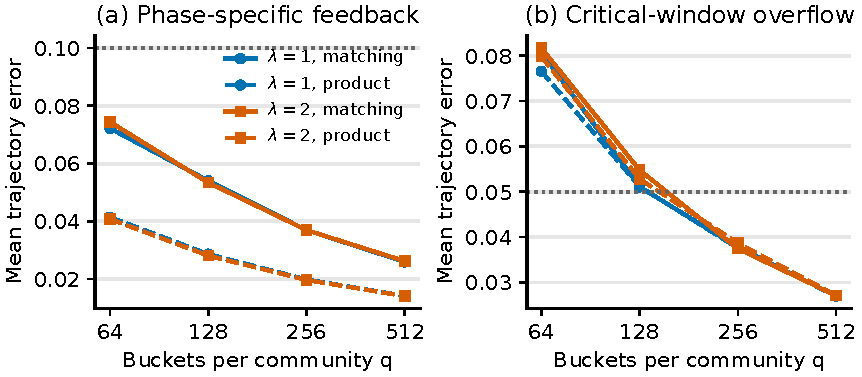
\includegraphics[width=\textwidth]{figures/finite_scale.pdf}
\caption{Descriptive finite-scale errors from the original saved outcomes.
Left: mean per-trajectory feedback RMS over 16 phases.
Right: mean per-trajectory maximum overflow error over five offsets.
Line styles distinguish matching and product kernels; markers distinguish
$\lambda=1,2$. The horizontal lines show the frozen per-trajectory margins,
not confidence limits for these plotted means. Shared labels are not pooled.
No convergence rate is fitted.}
\label{fig:finite}
\end{figure}

\subsection{Terminal diffusion and unconditional overflow}\label{sec:endtoend}
A separately frozen prospective batch has $q=512$, $\kappa=1$,
$\lambda=1,2$, and matching or product crosses. Its four cells each have
4096 labels. The labels are shared across cells, giving 16384 endpoints
rather than 16384 independent observations.
The targets are the unconditional mean difference
$\E[Z_c(q^2)/q]-\E[S_0(D_1)]$ and the Kolmogorov distance between
$\cL(\Delta_{q^2}/q)$ and $\cL(D_1)$.
The reference uses 32768 preserved SDE paths per $\lambda$, with 16384 Euler
steps per path. No observed microscopic imbalance enters its overflow mean.

\begin{figure}[t]
\centering
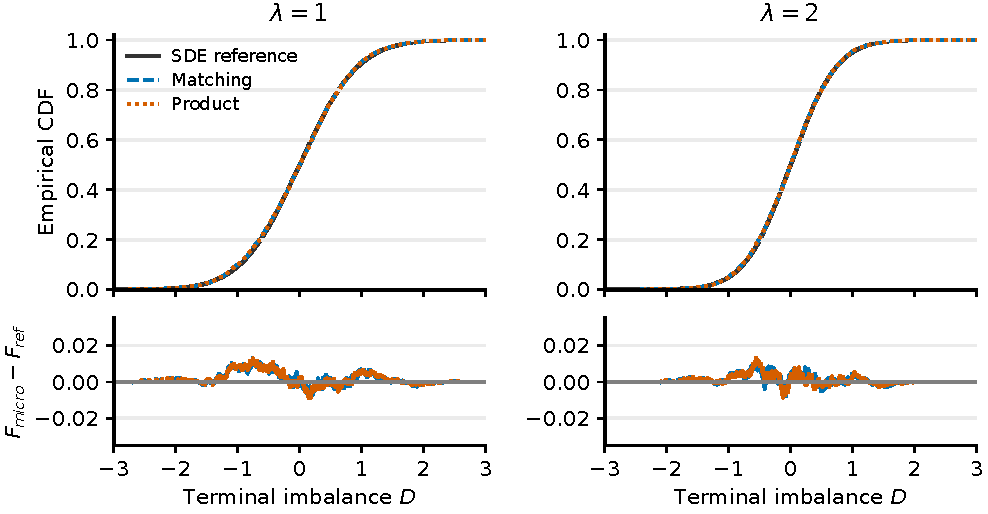
\includegraphics[width=\textwidth]{figures/terminal_law.pdf}
\caption{Terminal imbalance: the two prospective microscopic empirical CDFs
and the independently generated, preserved SDE reference for each $\lambda$.
The lower panels show microscopic minus reference empirical CDFs at all jumps.
Each microscopic cell has 4096 labels; each reference has 32768 paths.
The curves are descriptive; the numerical and sampling allowances enter the
distance bounds in Table~\ref{tab:prospective}.}
\label{fig:terminal}
\end{figure}

\begin{table}[t]
\caption{Prospective comparisons at $q=512$, $\kappa=1$.
Mean intervals bound microscopic mean overflow minus the SDE mean readout.
CDF upper bounds concern terminal imbalance and have lower bound zero.
All displayed limits are rounded outwards and include reference error.}
\label{tab:prospective}
\centering\small
\begin{tabular}{clcc}\toprule
$\lambda$ & Cross kernel & Mean-difference interval & CDF upper bound\\\midrule
1 & matching & $[-0.00840,\ 0.01010]$ & 0.06542\\
1 & product  & $[-0.00860,\ 0.00993]$ & 0.06500\\
2 & matching & $[-0.00663,\ 0.00844]$ & 0.07021\\
2 & product  & $[-0.00671,\ 0.00834]$ & 0.07119\\\bottomrule
\end{tabular}
\end{table}

All mean intervals lie within the frozen $[-0.05,0.05]$ margin.
All CDF upper bounds lie below the frozen $0.20$ margin.
The eight comparisons have joint failure allocation below $0.018138367441$,
giving at least $95\%$ coverage under the ideal input-word and reference-arithmetic
contracts in Supplement sections~\ref*{app:inference} and~\ref*{app:sdebudget}.
Coverage is unconditional over the reused reference and fresh data, in a separate
family from the original claims. It requires independent words across labels and
fresh streams independent of prior history. Pseudorandom reproducibility does
not prove these premises. The old reference has no saved register snapshot.

The two comparisons answer different questions. The readout comparison
isolates internal variation at an observed imbalance. The prospective comparison
assesses the predicted imbalance law and unconditional overflow mean.
Together they support the model's interpretation at the tested parameters;
they do not establish a finite-size rate or validation for every fixed kernel.

\FloatBarrier
\section{Discussion}
The critical law retains internal load variation and discards fixed
cross-endpoint correlations. Replacing a fixed matching by product sampling
preserves the leading overflow cost in this regime.
Corollary~\ref{cor:capacity} distinguishes order-$q$ expected overflow from
its order-$q^{-1}$ fraction. The internal profile determines that cost.

Complete-bipartite internal sampling supports label forgetting.
Double stochasticity supplies uniform cross marginals; integer loads and
left-favored ties enter nonexpansion and profile geometry.
Other graphs, adaptive sampling, and other tie rules require further arguments.
Effective profile tracking remains open. The finite-size comparisons cover
specified tolerances at $\kappa=1$, $\lambda=1,2$.

\paragraph{Data and code}
Frozen code, protocols, outputs, seeds, and logs are in the
\href{https://github.com/19991111/huaweipro-tpht-linux}{public repository}.
Supplement section~\ref*{app:artifact} lists immutable commits and audit limits.

\section*{AI assistance}
OpenAI's Codex assisted with literature searches, manuscript organization and
drafting, proof checking, code preparation for reanalysis of preserved outputs,
figure preparation, and document checks.
The author is responsible for the manuscript, including its mathematical claims,
references, code, and interpretation of results.
\bibliographystyle{siamplain}
\bibliography{references}
\end{document}
